% LaTeX path to the root directory of the current project
\providecommand{\econtexRoot}{}
\renewcommand{\econtexRoot}{..}
\providecommand{\econtexPaths}{LaTeX}\renewcommand{\econtexPaths}{\econtexRoot/LaTeX/econtexPaths}
\documentclass[\econtexRoot/BufferStockTheory]{subfiles}
% LaTeX path to the root directory of the current project
\providecommand{\econtexRoot}{}
\renewcommand{\econtexRoot}{..}
\providecommand{\econtexPaths}{LaTeX}\renewcommand{\econtexPaths}{\econtexRoot/LaTeX/econtexPaths}
\input{\LaTeXFiles/econtex_onlyinsubfile}
\onlyinsubfile{\externaldocument{BufferStockTheory}}

\begin{document}\label{sec:ApndxConditionDiagrams}
\hypertarget{ApndxConditionDiagrams}{}
\section{Relational Diagrams for the Inequality Conditions}

This appendix explains the paper's `inequalities' diagrams (\ref{fig:RelatePFGICFHWCRICPFFVAC},\ref{fig:Inequalities}).\footnote{Unless otherwise noted, the diagrams abide by the conventions that are used for constructing diagrams in \href{https://en.wikipedia.org/wiki/Diagram_(category_theory)}{category theory}.  In particular, the inequalities in the upper and lower triangular parts of the diagram indicate that this is not a commutative diagram.}


\subsection{The Unconstrained Perfect Foresight Model}


The basic idea is presented in Figure~\ref{fig:InequalityPFGICFHWCRIC}, whose three nodes represent values of the absolute patience factor $\Pat$, the permanent-income growth factor $\PGro$, and the riskfree interest factor $\Rfree$.  The arrows represent imposition of the labeled inequality condition  (like,  the uppermost arrow, pointing from {$\Pat$} to $\PGro$, reflects imposition of the {\PFGIC}).\footnote{For convenience, the equivalent ($\equiv$) mathematical statement of each condition is expressed nearby in parentheses.}

Traversal of the diagram is simple: Start at any node, and deduce a chain of inequalities by following any arrow that exits that node, and any arrows that exit from successive nodes, until reaching a point where no exit condition can be satisfied (that is, until the diagram defines no further inequalities).

Negation of a condition is also fairly simple.  The negation of the $\PFGIC$ is represented in the lower curved arrow pointing from $\PGro$ to {$\Pat$}, labeled \cncl{\PFGIC}.  The only outgoing arrow from $\Pat$ points to the {\RIC}, so the only further condition that the diagram maps is $\Pat > \Rfree$.  But imposing this condition allows us to conclude that $\PGro < \Rfree$ because $\PGro < \Pat$ and $\Pat < \Rfree$.  This illustrates the usefulness of the diagram: It can transparently show alternative ways to reach the same conclusion.  (Generically, if you start at $\PGro$ and end up at $\Rfree$ you know that the {\FHWC} holds).

Notationally, rather than showing both arrows for every condition ($\PFGIC$ and $\cncl{\PFGIC}$, say), it is simpler is to define a convention that negation of a condition is indicated by the reversal of the corresponding arrow.  So, for example, the negation of the {\RIC},  $\cncl{\RIC} \equiv \Pat > \Rfree$, would be represented by moving the arrowhead from the bottom right to the top left of the line segment connecting {$\Pat$} and $\Rfree$.

\begin{comment}
\begin{figure}
\centering
\subfigure[Transparent Version (with definitions)]{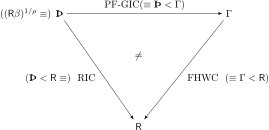
\includegraphics[width=6in]{\FigDir/InequalityPFGICFHWCRIC}}
\subfigure[Simplified Version (Same Content)]{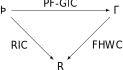
\includegraphics[width=4in]{\FigDir/InequalityPFGICFHWCRIC-Simple}}
\caption{Inequality Conditions for Perfect Foresight Model \\ (Start at a node and follow arrows)}
\label{fig:InequalityPFGICFHWCRIC}
\end{figure}
\end{comment}

Using this notation (and dropping the definitions) leads to the simpler diagram in part b of the diagram.  So, for example, if we were to start at the $\PGro$ node and impose $\cncl{\PFGIC}$ (reversing the arrow), we could traverse the diagram counterclockwise from $\PGro$ through $\Pat$ to $\Rfree$ and, as before, impose the {\RIC}, and reach the conclusion that $\PGro > \Rfree$.%  Traversal of the diagram stops upon reaching a node (like $\Rfree$) from which there are no exiting arrows.  (Traversal also must stop if it reaches any node from which the starting node could be reached (since a quantity cannot be strictly greater than itself))

So, if we were to start at $\Rfree$ and then impose $\cncl{\FHWC}$, that would reverse the arrow connecting $\Rfree$ and $\PGro$.  If we were then to impose $\cncl{\PFGIC}$, we would follow the arrow to {$\Pat$}.  But
\begin{equation}\begin{gathered}\begin{aligned}
  \cncl{\FHWC}:~~~~  \Rfree & < \PGro \notag  
  \\ \cncl{\PFGIC}:~~~~ \PGro & < \Pat %~\left(\equiv (\Rfree \DiscFac)^{1/\CRRA}\right)
                                \label{eq:cnclRIC}
  \\ \Rightarrow \cncl{\RIC}:~~~~\Rfree & < \Pat \notag,
\end{aligned}\end{gathered}\end{equation}
so in this case reversing two arrows requires reversal of the third.

% which illustrates another aspect of the diagram: If all arrows are reversed in a partial traversal of the diagram leading to a final step, then the arrow for the final step must also be reversed.  In this case, since both conditions leading to $\Rfree$ have had their arrows reversed, the arrow coming out of $\Rfree$ should also be reversed, implying the negation of the {\RIC} -- as \eqref{eq:cnclRIC} proved.

% For clarity, further diagrams will omit multiple arrows indicating reversal of causality (in Figure~\ref{fig:InequalityPFGICFHWCRIC} there would, for example, be only a single arrow, from {$\Pat$} to $\PGro$, at the top level of the diagram).  And definitions of conditions will also be omitted henceforth.

Under these conventions, the main text presents a version of the (simplified) diagram as extended to incorporate the $\PFFVAC$ \href{https://econ-ark.github.io/BufferStockTheory/#RelatePFGICFHWCRICPFFVAC}{in Figure}~\ref{fig:RelatePFGICFHWCRICPFFVAC}).\footnote{For readers familiar with the \href{https://en.wikipedia.org/wiki/Commutative_diagram}{commutative diagrams}, it should be noted that despite the similar appearance, this diagram is not exactly commutative.}%  because the three ways of arriving at the conclusion embodied in the diagonal arrow (the {\PFFVAC}) are NOT identical in their other implications.}

\providecommand{\figName}{}
\renewcommand{\figName}{RelatePFGICFHWCRICPFFVAC}
\providecommand{\figFile}{\figName}
\input{\FigDir/\figName}

This diagram can be interpreted, for example, as saying  that, starting at the $\Pat$ node, it is possible to derive the $\PFFVAC$\footnote{in the form $\Pat < (\Rfree/\PGro)^{1/\CRRA}\PGro$} by imposing both the {\PFGIC} and the {\FHWC}; or by imposing {\RIC} and \cncl{\FHWC}.  Or, starting at the $\PGro$ node, we can follow the imposition of the {\FHWC} (twice - reversing the arrow labeled $\cncl{\FHWC}$) and then $\cncl{\RIC}$ to reach the conclusion that $\Pat < \PGro$.  Algebraically,
\begin{equation}\begin{gathered}\begin{aligned}
  {\FHWC}:~~~ \PGro & < \Rfree 
  \\ \cncl{\RIC}:~~~ \Rfree & < \Pat 
  \\ \PGro & < \Pat \label{eq:cnclPFGIC}
\end{aligned}\end{gathered}\end{equation}
which leads to the negation of both of the conditions leading into $\Pat$.  \cncl{\PFGIC} is obtained directly as the last line in \eqref{eq:cnclPFGIC} and \cncl{\PFFVAC} follows if we start by multipling the Return Patience Factor ({\RPF}=$\Pat/\Rfree$) by the \FHWF (=$\PGro/\Rfree$) raised to the power $1/\CRRA-1$, which is negative since we imposed $\CRRA > 1$.  {\FHWC} implies {\FHWF} $< 1$ so when {\FHWF} is raised to a negative power the result is greater than one.
Multiplying the {\RPF} (which exceeds 1 because \cncl{\RIC}) by another number greater than one yields a product that must be greater than one:
\begin{equation}\begin{gathered}\begin{aligned}
  1  & < \overbrace{\left(\frac{(\Rfree \DiscFac)^{1/\CRRA}}{\Rfree}\right)}^{>1 \text{~from~}\cncl{\RIC}}\overbrace{\left(\PGro/\Rfree\right)^{1/\CRRA-1}}^{\phantom{...}>1~\text{~from~} \FHWC} \notag
  \\ 1  & < \left(\frac{(\Rfree \DiscFac)^{1/\CRRA}}{(\Rfree/\PGro)^{1/\CRRA}\Rfree\PGro/\Rfree}\right) \label{eq:cnclFHWFAndcnclRICImplycnclPFFVAC}
  \\ \Rfree^{1/\CRRA}\PGro^{1 - 1/\CRRA} = (\Rfree/\PGro)^{1/\CRRA} \PGro  & < \Pat \notag
\end{aligned}\end{gathered}\end{equation}
which is one way of writing $\cncl{\PFFVAC}$.

The complexity of this algebraic calculation illustrates the usefulness of the diagram, in which one merely needs to follow arrows to reach the same result.

After the warmup of constructing these conditions for the perfect foresight case, we can represent the relationships between all the conditions in both the perfect foresight case and the case with uncertainty as shown in Figure~\ref{fig:Inequalities} in the paper (reproduced below).

\renewcommand{\figName}{Inequalities} % Allows generic definition of hypertargets based on title of figure
\renewcommand{\figFile}{\figName} %  and on filename
\hypertarget{\figFile}{}
\hypertarget{\figName}{}
\input{\FigDir/\figName} % Read in the tex to generate the figure


\end{document}


% Local Variables:
% eval: (setq TeX-command-list  (assq-delete-all (car (assoc "BibTeX" TeX-command-list)) TeX-command-list))
% eval: (setq TeX-command-list  (assq-delete-all (car (assoc "BibTeX" TeX-command-list)) TeX-command-list))
% eval: (setq TeX-command-list  (assq-delete-all (car (assoc "BibTeX" TeX-command-list)) TeX-command-list))
% eval: (setq TeX-command-list  (assq-delete-all (car (assoc "BibTeX" TeX-command-list)) TeX-command-list))
% eval: (setq TeX-command-list  (assq-delete-all (car (assoc "Biber"  TeX-command-list)) TeX-command-list))
% eval: (add-to-list 'TeX-command-list '("BibTeX" "bibtex ../LaTeX/%s" TeX-run-BibTeX nil t                                                                              :help "Run BibTeX") t)
% eval: (add-to-list 'TeX-command-list '("BibTeX" "bibtex ../LaTeX/%s" TeX-run-BibTeX nil (plain-tex-mode latex-mode doctex-mode ams-tex-mode texinfo-mode context-mode) :help "Run BibTeX") t)
% TeX-PDF-mode: t
% TeX-file-line-error: t
% TeX-debug-warnings: t
% LaTeX-command-style: (("" "%(PDF)%(latex) %(file-line-error) %(extraopts) -output-directory=../LaTeX %S%(PDFout)"))
% TeX-source-correlate-mode: t
% TeX-parse-self: t
% eval: (cond ((string-equal system-type "darwin") (progn (setq TeX-view-program-list '(("Skim" "/Applications/Skim.app/Contents/SharedSupport/displayline -b %n ../LaTeX/%o %b"))))))
% TeX-parse-all-errors: t
% End:
